\chapter{Evaluierung}
	Welche Software und welche speziellen Hardwaremodule bezüglich des Projekts benutzt werden sollten wurde im Voraus festgelegt und an dieser Stelle entsprechend der Auswahl vorgestellt.
	\section{Software}
		\subsection{Entwicklungsumgebung}
			Bezüglich des Mikrocontrollers \enquote{mbed NXP LPC1768} wird vom mbed-Projekt eine Online-Entwicklungsumgebung bereitgestellt, die im Projekt verwendet werden sollte.
			
			Die Entwicklungsumgebung bietet:
			
			\nomenclature{SDK}{Software Development Kit}
			\begin{itemize}
				\item High level C/C++ SDK
				\item Kochbuch mit publizierten Bibliotheken und Projekten
				\item Editer mit Code-Highlighting
				\item Projektbaumverwaltung
				\item Compiler
				\item Versionsverwaltung Mercurial
			\end{itemize}
			
			Weiterhin kann das Projekt aus der Entwicklungsumgebung sehr einfach in andere Umgebungen exportiert, beziehungsweise von diesen importiert werden. Zu diesen Umgebungen zählen unter anderem die \enquote{GCC ARM Embedded} und die \enquote{GCC Code Sourcery}.
			
			Zum Projekt selbst werden auf einer Übersichtsseite mehrere Fakten zusammengetragen. Diese enthalten unter anderem, ob die importierten Bibliotheken auf dem aktuellen Stand sind und wie die Speichernutzung auf der aktuellen Plattform aussieht.
		\subsection{Bibliotheken}
			Die vom mbed-Projekt und seinen Nutzern bereitgestellten Bibliotheken sind sehr umfangreich. Bereits die Standardbibliothek macht das arbeiten mit dem Controller sehr einfach und im Vergleich zu anderen Mikrocontrollern ist diese Bibliothek als sehr Benutzerfreundlich einzustufen.
			
			Die Standardbibliothek fasst alle Dinge zusammen, die am Controller selbst eingestellt werden können. Soll beispielsweise ein Pin als \enquote{Output-Pin} definiert werden, ist dies über diese Bibliothek möglich. Auch die höheren Funktionen, wie die I$^{2}$C Benutzung, stellt diese Bibliothek bereit.
			
			Zusätzlich zur Standardbibliothek wurde im Projekt die Bibliothek \enquote{RTOS} benutzt. Diese stellt eine Implementierung eines Echtzeit-Betriebssystems dar, das viele Dinge auf einem Mikrocontroller vereinfacht. Von der Bibliothek wird unter anderem bereitgestellt:
			
			\begin{itemize}
				\item Thread-Modell mit Scheduler
				\item Inter-Prozess-Kommunikation
				\item Semaphore
				\item Interrupt-Service-Routinen
				\item Signale
				\item Speicher-Pools
			\end{itemize}
			
			In der vorliegen Arbeit wurde dabei Gebrauch vom Thread-Modell, den Sempahoren und den Interrupt-Service-Routinen gemacht.
			
			\cite{RTOS}
	\section{Hardware}
		\subsection{Mikrocontroller \enquote{mbed NXP LPC1768}}
			Der Mikrocontroller wurde vom mbed-Projekt der Firma ARM Holdings plc bereitgestellt. Er ist dafür gedacht eine schnelle Prototypen-Entwicklung auf einer, für einen Mikrocontroller leistungsfähigen Plattform durchführen zu können.
			
			Der benutzte Mikrocontroller ist die größte Ausbaustufe der erhältlichen Prototyp-Module. In der folgenden \enquote{Feature-List} \cite{LPC1768} und der Abbild \ref{fig:LPC1768-pinout} ist kurz aufgeführt, was der Controller bereitstellt.
			
			\begin{itemize}
				\item High performance ARM® Cortex™-M3 Core
				\item 96MHz, 32KB RAM, 512KB FLASH
				\item Ethernet, USB Host/Device, 2xSPI, 2xI$^{2}$C, 3xUART, CAN, 6xPWM, 6xADC, GPIO
				\item 40-pin 0.1" pitch DIP package, 54x26mm
				\item 5V USB or 4.5-9V supply
				\item Built-in USB drag 'n' drop FLASH programmer
			\end{itemize}
			
			\begin{figure}[H]
				\centering
				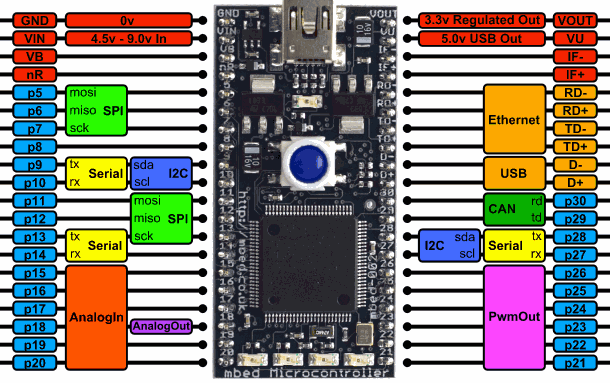
\includegraphics[width=0.7\linewidth]{Grafiken/LPC1768-pinout}
				\caption[mbed NXP LPC1768 Pinout]{mbed NXP LPC1768 Pinout\protect\footnotemark}
%				\caption[TI Beispiel zum Schedulerverhalten]{TI Beispiel zum Schedulerverhalten\protect\footnotemark}
				\label{fig:LPC1768-pinout}
			\end{figure}
			\footnotetext{Quelle: \cite{LPC1768}}
			
			\cite{LPC1768}
		\subsection{Empfangsmodul DCF77}
			Das im Projekt benutzte Empfangsmodul \enquote{C-Control DCF-Empfängerplatine} besteht aus einer fertigen Schaltung zum Empfang des DCF77-Signals. Verbaut ist eine Ferritkernantenne, welche an einer Schaltung befestigt ist, die das empfangene Signal auswertet und an zwei Ausgängen als Logikpegel entsprechend der Versorgungsspannung ausgibt. Da diese Ausgänge jedoch offene Kollektoren sind und nur mit 1 mA belastet werden können, muss gegebenenfalls eine Vorschaltung errichtet werden, die das Signal für einen Mikrocontroller aufwertet.
			
			\newpage
			Die technischen Daten des Empfängers sind:
			
			\begin{itemize}
			 \item Versorgungsspannung 2,5 bis 15 V DC
			 \item Stromaufnahme 3 mA
			 \item Ausgabe: Signal, Signal invertiert
			 \item Signalausgänge sind offene Kollektoren die maximal mit 30 V, 1 mA belastet werden können
			\end{itemize}
			
			\begin{figure}[H]
				\centering
				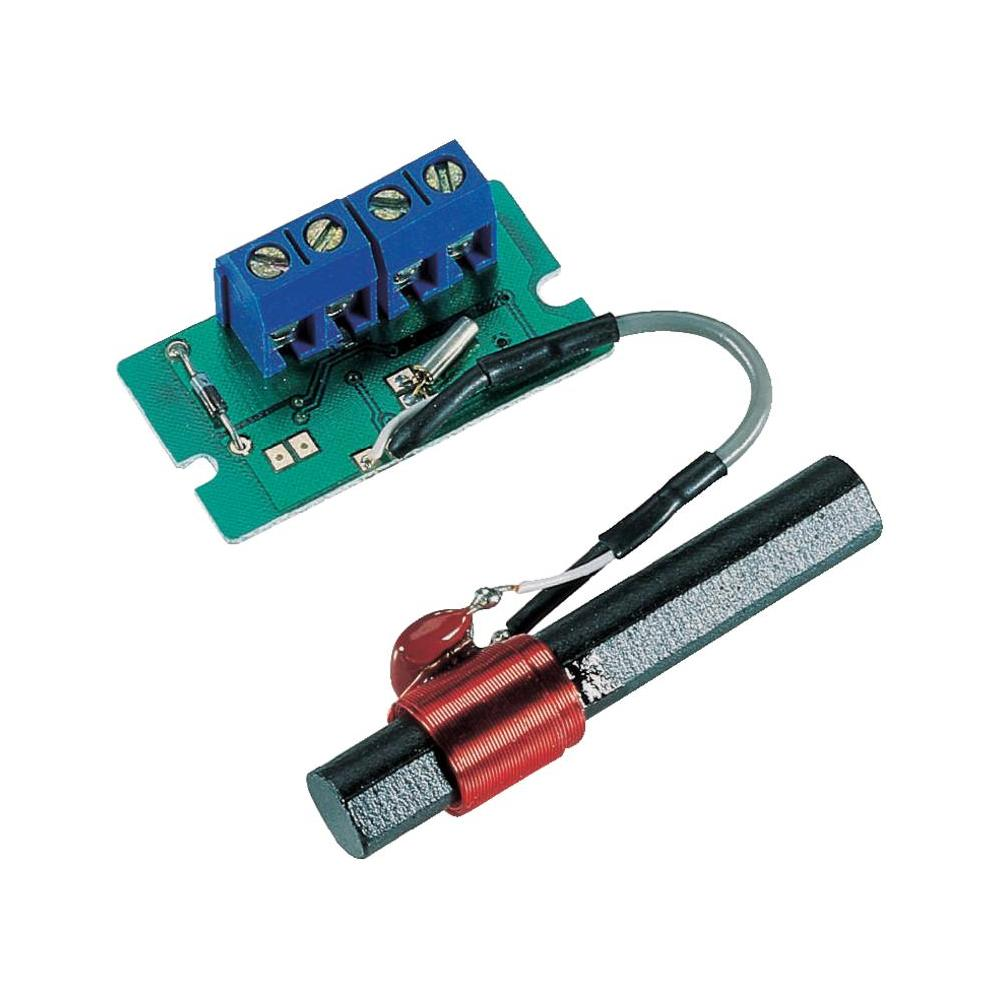
\includegraphics[width=0.6\linewidth,height = 8cm]{Grafiken/DCF77}
				\caption[DCF77 Antenne und Platine]{DCF77 Antenne und Platine\protect\footnotemark}
				\label{fig:DCF77}
			\end{figure}
			\footnotetext{Quelle: \cite{DCF77}}
			
			\cite{DCF77}, \cite{DCF77Manual}
		\subsection{Temperatur-/Feuchtigkeitssensor HYT2x1}
			\subsubsection{Daten zum HYT271/241}
				\begin{figure}[H]
				\centering
				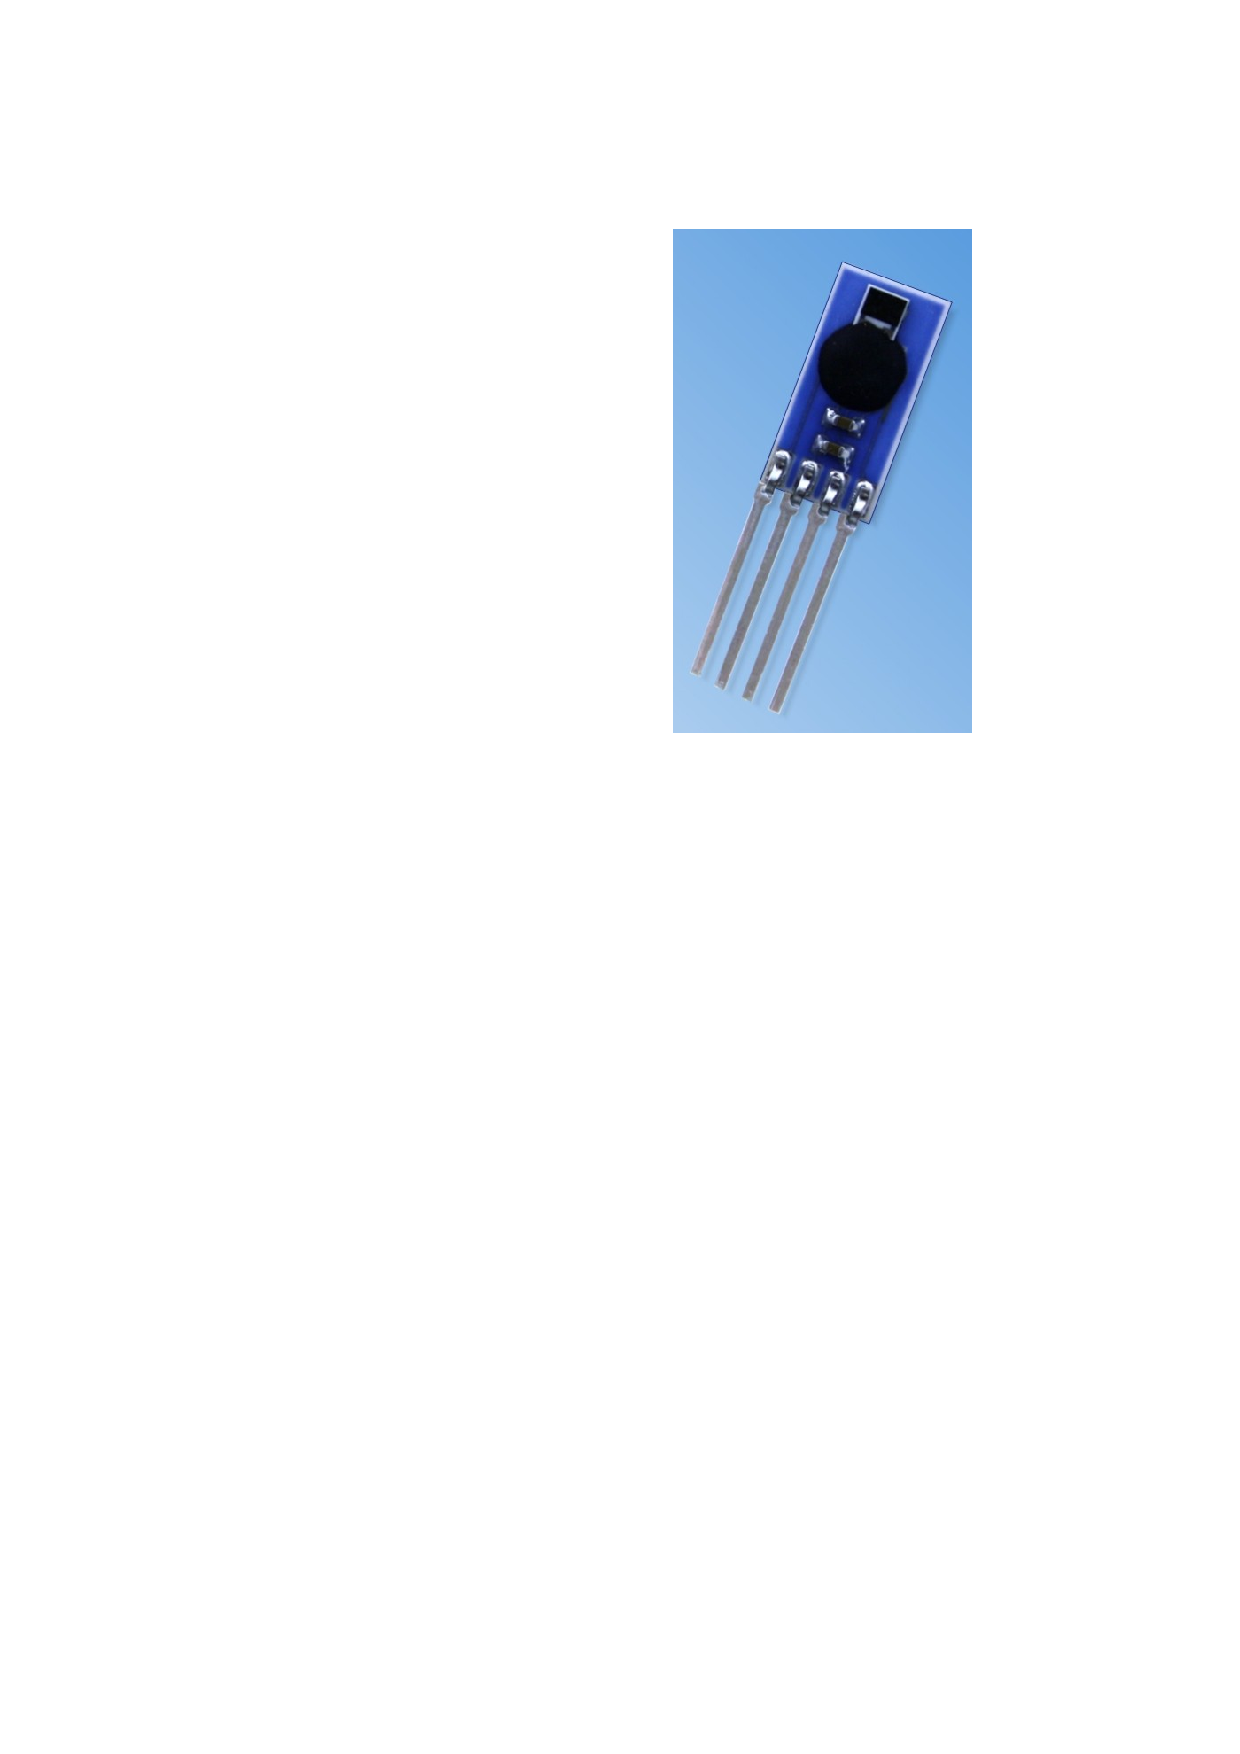
\includegraphics[height=5cm]{./Grafiken/HYT271}
				\caption[HYT271]{HYT271\protect\footnotemark}
				\label{fig:HYT271}
				\end{figure}
				\footnotetext{Quelle: \cite{HYTManual}}
				
				Bei den Sensoren HYT271 und HYT241 handelt es sich um Temperatur- und Feuchtigkeitssensoren mit einem gemeinsamen Messbereich bezüglich der Temperatur von -40$^{\circ}$C bis 125$^{\circ}$C. Die im Datenblatt angegebene Ungenauigkeit beträgt 0,2$^{\circ}$C, welche allerdings von der Temperatur abhängig ist. Die Abbildung \ref{fig:Genauigkeit_Temp} zeigt diesen Temperaturabhängigkeitsverlauf.
				
				\begin{figure}[H]
					\centering
					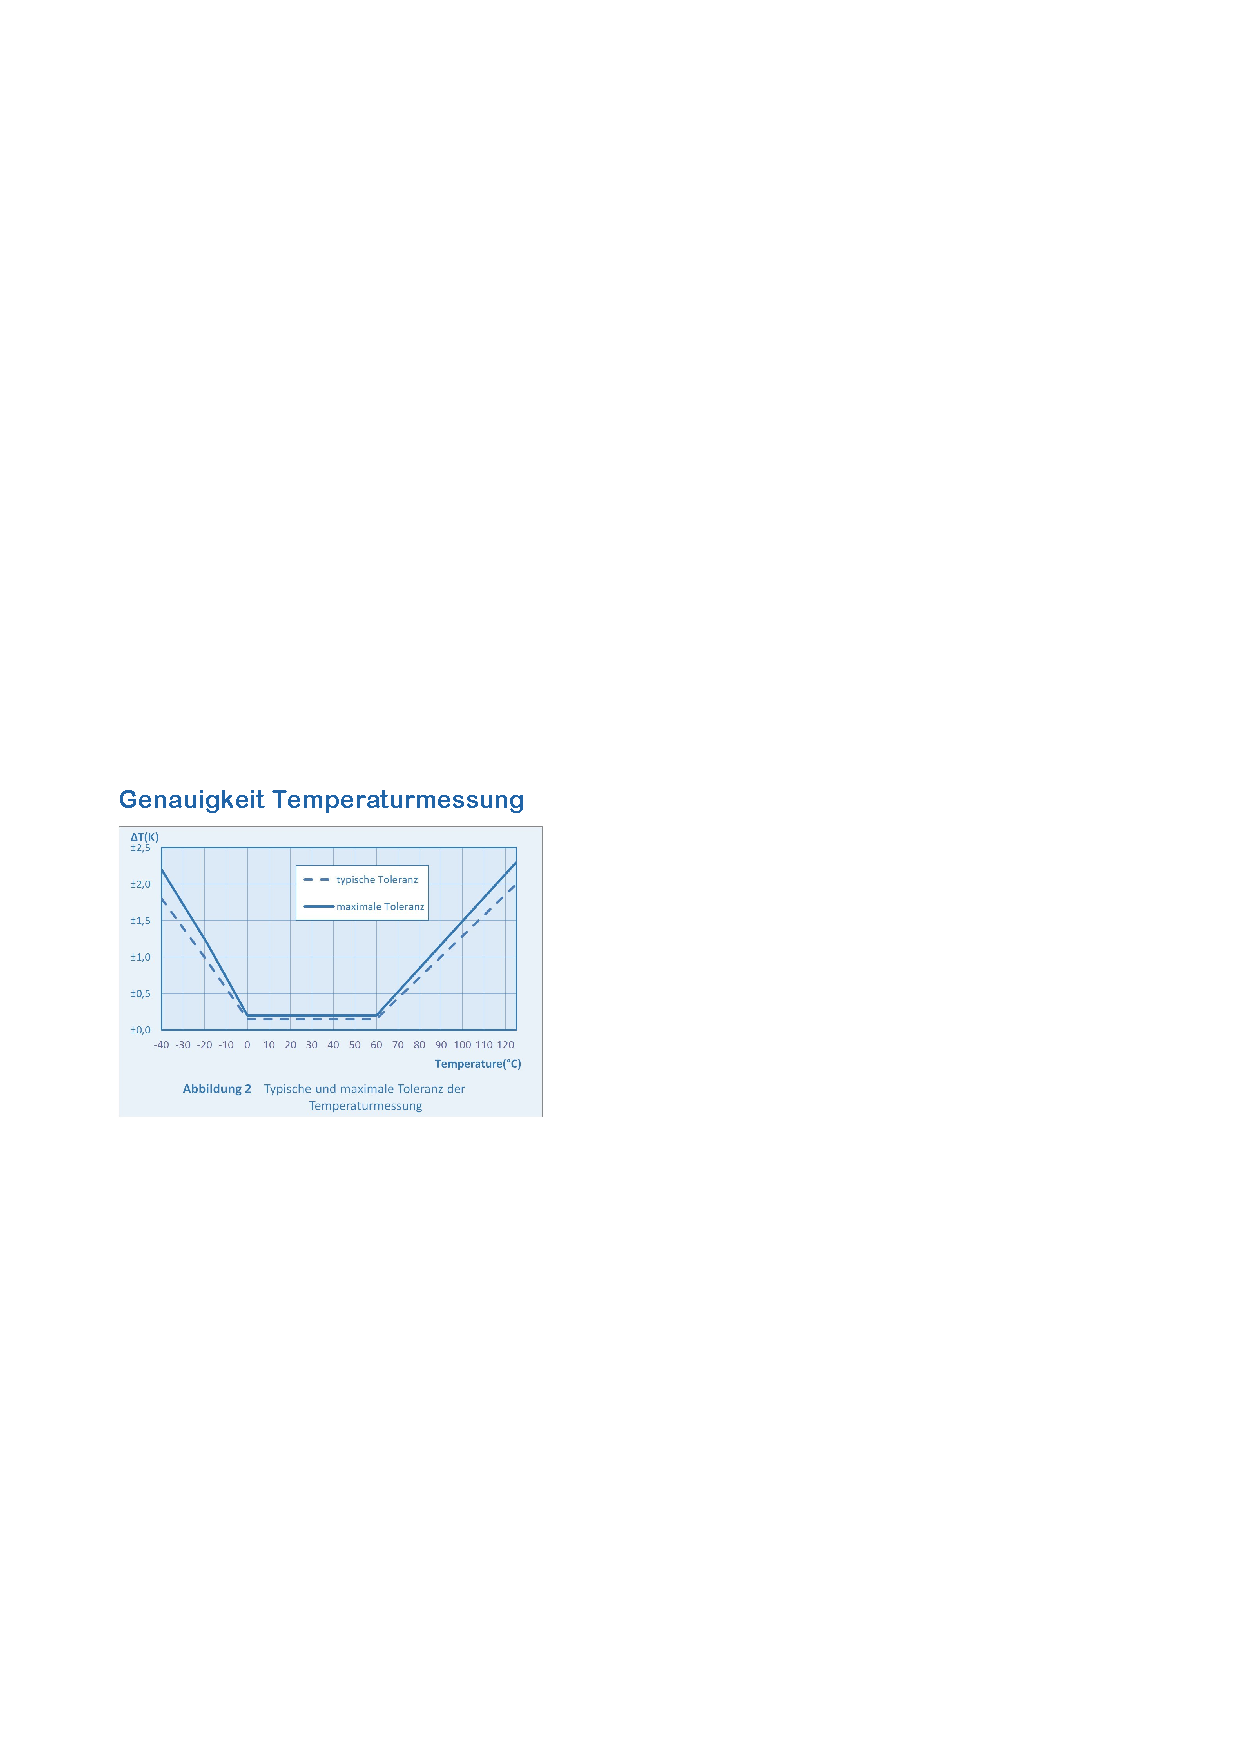
\includegraphics{./Grafiken/GenauigkeitTemp}
					\caption[Verlauf der Genauigkeit der Temperatur]{Verlauf der Genauigkeit der Temperatur\protect\footnotemark}
					\label{fig:Genauigkeit_Temp}
				\end{figure}
				\footnotetext{Quelle: \cite{HYTManual}}
				
				Der Messbereich der Feuchtigkeit beträgt 0\% bis 100\% relative Luftfeuchte. Auch hier existiert eine Ungenauigkeit, die ist mit 1,8\% angegeben ist. Die Feuchtigkeit unterliegt jedoch dem selben Effekt, dem auch die Temperatur unterliegt, der in Abbildung \ref{fig:Genauigkeit_Feuchte} dargestellt ist.
				
				\begin{figure}[H]
					\centering
					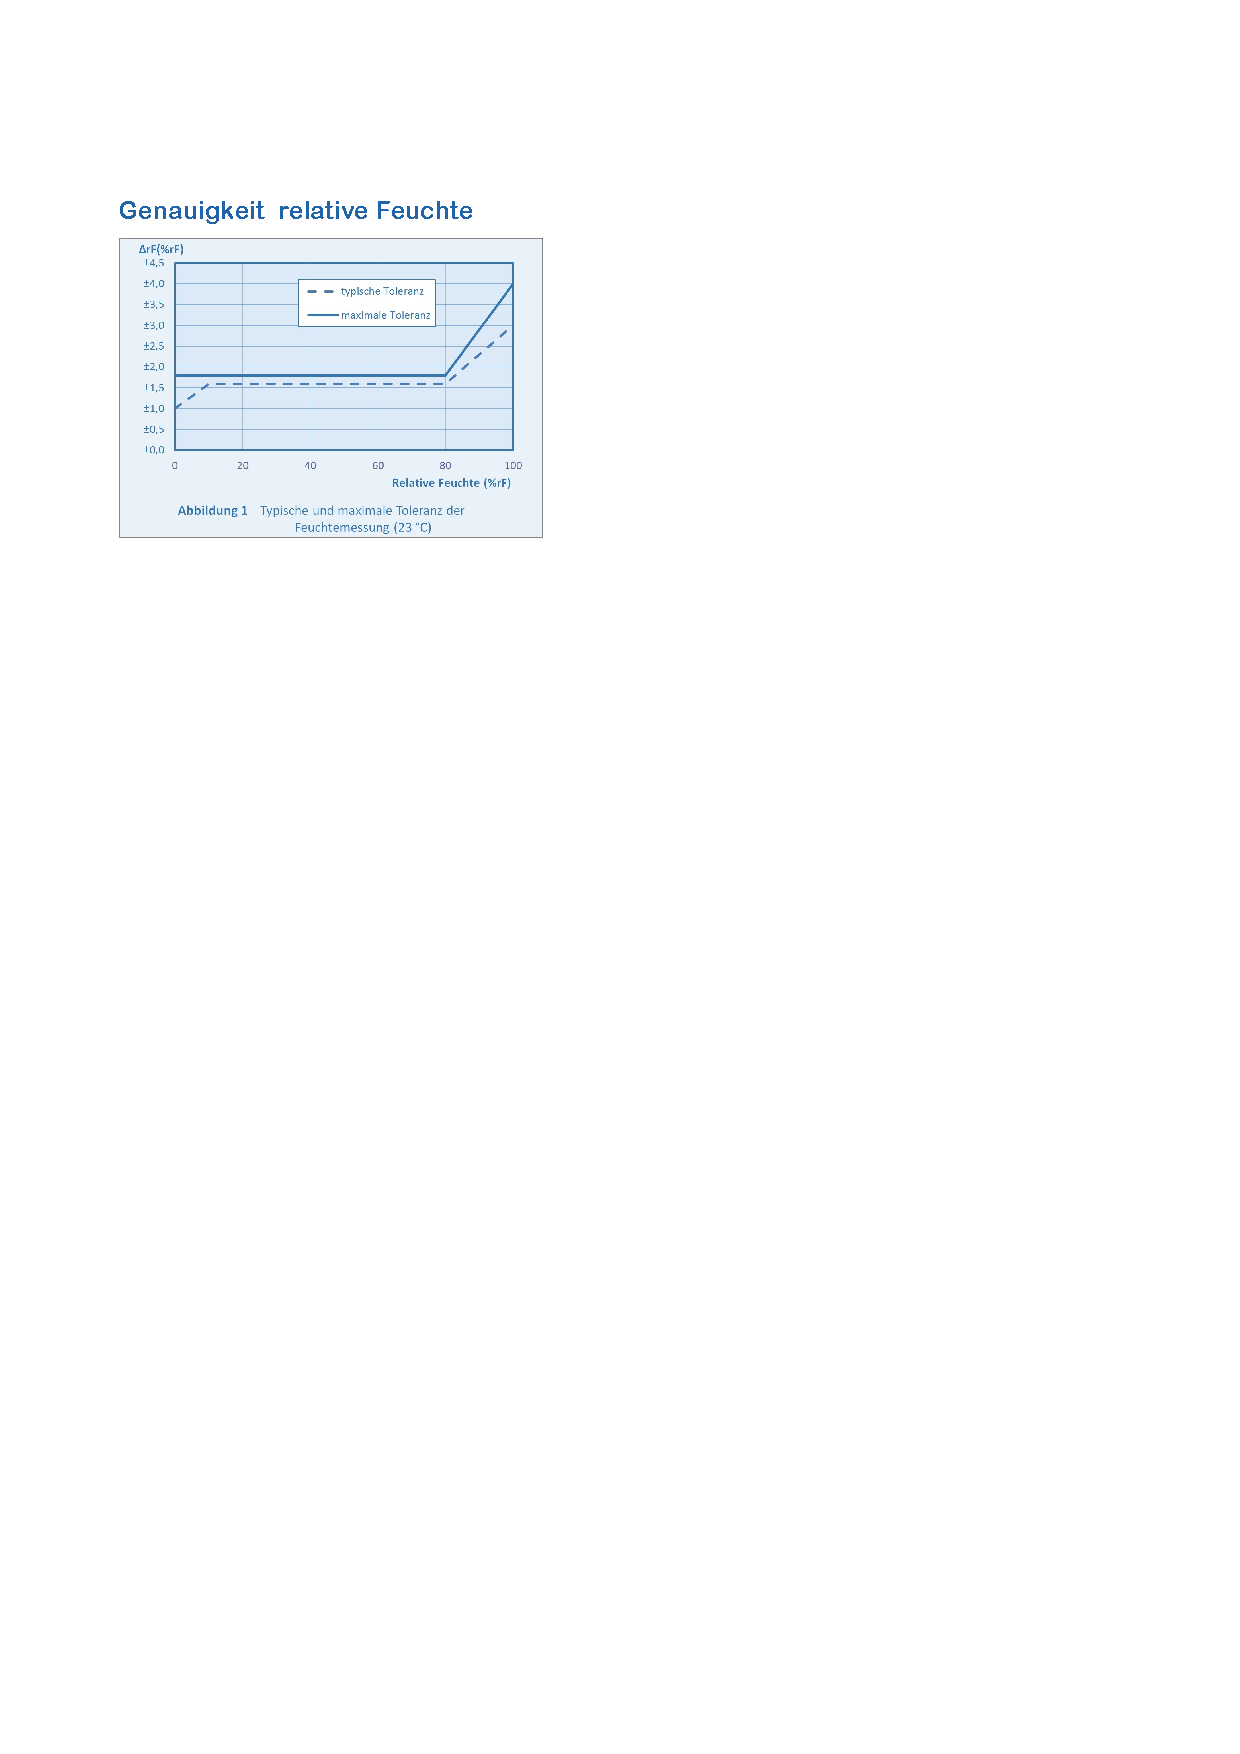
\includegraphics{./Grafiken/Genauigkeit_Feuchte}
					\caption[Verlauf der Genauigkeit der Feuchte]{Verlauf der Genauigkeit der Feuchte\protect\footnotemark}
					\label{fig:Genauigkeit_Feuchte}
				\end{figure}
				\footnotetext{Quelle: \cite{HYTManual}}
				
			\subsubsection{Technische Daten}
				\begin{table}[H]
					\centering
					\begin{tabular}{|l|l|}
					\hline Betriebsspannung & 2,7 bis 5,5 V \\
					\hline Stromaufnahme (Ruhezustand) & 1 $\mu$A \\
					\hline Stromaufnahme (Betrieb) & 850 $\mu$A \\
					\hline Schnittstellen & I²C \\
					\hline Anschlussleitungen & VCC, GND, SDA und SCL\\
					\hline
					\end{tabular}
					\caption{Technische Daten der Temperatur-/Feuchtigkeitssensoren}
					\label{table:TechHYT}
				\end{table}
			\subsubsection{Das HYT2x1 Interface}
				Die HYT271 und HYT241 Sensoren sind I$^{2}$C Slaves. Ihr Befehlssatz ist gering, aber ausreichend. Es stehen 2 Befehle zur Kommunikation zur Verfügung.
				
				\begin{description}
				\item[Measuring Request (MR)] Beim Mesuring Request wird nur auf die Adresse des Geräts geschrieben. Es müssen dabei keine Daten übertragen werden. Der reine Schreib-Befehl reicht aus.
				\item[Data Fetch (DF)] Bei Data Fetch handelt es sich um einen Lesebefehl. Hierzu muss auf den Bus die Adresse des Sensors und eine abschließende 0 gelegt werden. Folgend können vom Sensor 4 Byte empfangen und in Temperatur und Feuchtigkeit umgerechnet werden. Zwischen Data Fetch und Measuring Request sollten ca. 50ms Zeit vergehen, da sonst beim Data Fetch nur die bei vorherigen Messung ausgelesenen Werte übertragen werden.
				\end{description}
				
			\subsection{Regensensor CON-REGME-24V}
				Der vom Unternehmen B+B Thermo erworbene Sensor misst über eine mäanderförmige Leiterplatte an der Oberfläche des Moduls die Impedanz und kann daraus detektieren, ob Niederschlag vorherrscht oder nicht. Verändert sich die Leitfähigkeit zwischen den Mäandern positiv, so kann angenommen werden das es Niederschlag gibt.
				
				\newpage
				Besteht Niederschlag, so schließt oder öffnet der Sensor eigenständig ein potentialfreies Relais. Dies kann als Signalquelle frei genutzt werden. Zu beachten ist jedoch, dass keine Netzspannung mit diesem Relais geschaltet werden kann.
				
				Je nach Konfiguration des Sensors schaltet sich bei Niederschlag eine Heizung zu, die die Sensoroberfläche erwärmt. Dadurch verdunstet eventuell aufliegender Niederschlag und das Messergebnis wird deutlich genauer, da früher ein Ende des Niederschlags detektiert werden kann. Sinnvoll ist die Heizung ebenfalls im Winter, damit die Sensoroberfläche nicht vereist.
				
				Am Sensormodul selbst können noch verschiedene Einstellungen getroffen werden. Diese sind:
				
				\begin{itemize}
					\item Bei Niederschlag das Relais schließen oder öffnen
					\item Heizung verwenden oder nicht
					\item Ein optional angeschlossenes Piezoelement bei Niederschlag ertönen lassen oder abschalten
				\end{itemize}
				
				Die wichtigsten technischen Daten des Moduls sind wie folgt und können nochmals genau in dem im Lieferumfang beigelegten Datenblatt nachgelesen werden.
				
				\begin{table}[H]
					\centering
					\begin{tabular}{|l|l|}
						\hline Betriebsspannung &  24 V DC/AC +10\% \\ 
						\hline Stromaufnahme & 50 mA, Heizung 40-180 mA \\ 
						\hline Messverfahren & elektrolytische Wechselspannungsmessung \\ 
						\hline Belastung der Kontakte & max. 30 V DC / 4 A \\ 
						\hline Anschlussklemmen & 0,5 mm² - 1,5 mm² \\ 
						\hline Maße & 80 x 82 x 58 mm \\
						\hline 
					\end{tabular}
					\caption{Technische Daten des Regensensors}
					\label{table:TechRain}
				\end{table}
				
				\cite{Rain}